%!TEX root = spack-sc15.tex

\subsection{Versioned Virtual Dependencies}\label{sec:virtual}

\begin{figure}
	\begin{minted}[numbersep=5pt,
	              fontsize=\scriptsize,
	              frame=lines,
                  framesep=2mm]{python}
 # providers of mpi                       # mpi dependents
 class Mvapich2(Package):                 class Mpileaks(Package):
     provides('mpi@:2.2', when='@1.9')        depends_on('mpi')
     provides('mpi@:3.0', when='@2.0')           ...
     ...                                  class Gerris(Package):
 class Mpich(Package):                        depends_on('mpi@2:')
     provides('mpi@:3', when='@3:')           ...
     provides('mpi@:1', when='@1:')
     ...
\end{minted}
\caption{
	Virtual dependencies.
	\label{fig:virtual-deps}
}
\end{figure}

\begin{figure*}[ht!]
	\centering
	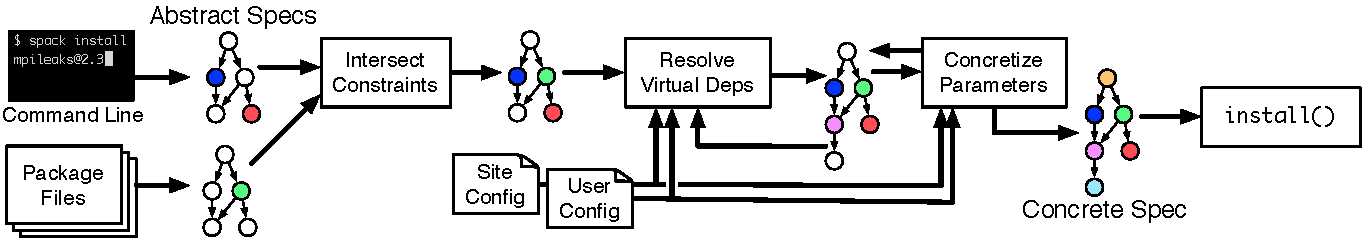
\includegraphics[width=.9\textwidth]{figs/concretization.pdf}
	\caption{
		Spack's concretization process.
		\label{fig:concretization}
	}
\end{figure*}


Many libraries share a common interface and can be interchanged within a build.
The archetypal examples in HPC are MPI libraries, which has several
open source (e.g., MPICH, OpenMPI, and MVAPICH) and 
vendor-specific implementations. An application that can be built with 
one MPI implementation can generally be
built with another.  Another example is the Basic Linear Algebra
Subroutines (BLAS), which has many fungible implementations
(e.g., ATLAS, LAPACK-BLAS, and MKL).

Neither MPI nor BLAS has a standard ABI, so applications cannot simply be
re-linked with a new version. They must be recompiled and reinstalled.
At LLNL, we must frequently build tools with many versions of MPI to support
the many different applications that run at our center.
Complicating matters, the MPI interface is versioned, and some
packages need later versions of MPI to run correctly.  Often, MPI
{\it implementation} versions do not correspond obviously to MPI
interface versions, and determining the right version of
MPI to pair with an application can be tedious and tricky.

To allow rapid composition of libraries using an interface, Spack supports
{\it virtual dependencies}.  A virtual dependency is an abstract name that
represents a library interface (or capability) instead of a library
implementation.  Packages that need this interface do need not to depend on
a specific implementation; they can depend on the virtual name, for which
the user or Spack can select an implementation at build time.
Other package managers support the notion of virtual dependencies, but Spack
adds {\it versioning} to its interfaces, which directly supports concepts 
like MPI versions and BLAS levels.  Spack
handles the details of managing and checking complex versioning constraints.

Figure~\ref{fig:virtual-deps} shows how packages provide
virtual interfaces in Spack.  The spec syntax concisely associates ranges 
of {\tt mpi} versions for the {\tt mvapich2} and {\tt mpich} packages.
The {\tt mpileaks} package requires {\tt mpi}, but it does not constrain the version.
Any version of {\tt mvapich2} or {\tt mpich} could be used to to satisfy the {\tt mpi}
constraint. The Gerris computational fluid dynamics library, however, needs MPI version 2 or higher.  So any
version except {\tt mpich} 1.x could be used to satisfy the constrained dependency.


%{\bf Dependencies.}
%Lines 6 and 7 in the table show the key feature that enables Spack's flexibility.
%The user can specify all of the above information not only for the package being
%installed, but also for its {\it dependencies}.  To do this, the user needs only supply
%\verb|^| and the dependency's name.  If we need to build a new version with a specific
%version of {\tt mvapich2}, we can simply add, e.g., \verb|^mvapich2@1.9|
%to the spec, and it will build with that MPI version instead of the default.
%This can also be done for multiple libraries in the same spec (line 7).
